We identified a list of primitives at different semantic levels useful to describe, design and author applications for SCL supported by smart objects and TUIs:

\begin{figure}[htb]
\centering
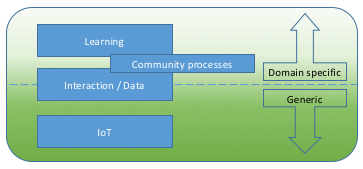
\includegraphics[width=8cm]{img/primitive_layers}
\caption{Semantic layers of the primitives.}
\label{fig:layers}
\end{figure}


\subsection{Generic level}
\medskip

\subsubsection{PHYSICAL MANIPULATION}
\begin{description}
\item [Touch] as the ability to detect finger interactions like a simple touch, swipes, multiple taps et simila;
\item [Multi-axial rotation] detects with sufficient precision object rotation and tilt;
\item [Shake and displacement] intended as the ability to detect when the object is shaken vigorously or is being physically moved.
\end{description}

\subsubsection{FEEDBACK AND OUTPUT}
\begin{description}
\item [Led light] can be used as a low fidelity output, more complex communication strategies can be implemented, like blinking, color fading and led matrix;
\item [Haptic] defined as vibration pattern that differ in intensity and duration;
\item [Sound] intended as simple beeping or composition of multi-tone sounds.
\end{description}

\subsubsection{OBJECT AUGMENTATION}
\begin{description}
\item [Untethered operation] augmented object should work independently and autonomously, without being hooked to any external device that provides connectivity or power support;
\item [Easily embeddable] technology should be easy to integrate into objects, without altering the original function and nature of the object;
\item [Energy autonomous] the objects should be as much autonomous as possible, effective energy usage, battery efficiency and energy harvesting can help at this regard.
\end{description}


\subsection{``Generic/Domain Specific'' overlapping level}
\medskip

\subsubsection{DATA}
\begin{description}
\item [Sensor data collection] intended as the opportunity to employ data gathered in real time from the surrounding ambient;
\item [Data visualization] as the ability to support visualization of simple information through low fidelity output;
\item [Data processing] involves elaboration of data coming from sensors and/or from third party services.
\end{description}

\subsubsection{INTERACTION STRATEGIES}
\begin{description}
\item [Object sharing] smart objects should be physically shareable, retaining their physical behavior. Augmenting the object with technology should not restrict its original affordances.
Background/foreground: interaction should be possible when the object is in the center of attention, but also when in background, providing context information possibly through glances and nudging;
\item [Distributed] interaction with several augmented objects orchestrated as a single user interface;
\item [Multimodal] object interaction based on more than one strategy, e.g. touch and speech recognition on the same object;
\item [Sensor based] it's an enabler for physical manipulation, since smart objects do not provide a dedicated interaction interface (like a keyboard or buttons), the interaction happens with the object itself.
\end{description}


\subsection{Domain Specific level}
\medskip

\subsubsection{LEARNING}
\begin{description}
\item [Reflection] occurs when reflecting on previous experience and behaviours;
\item [Behaviour change] the explicit goal is to modify or improve a specific behaviour;
\item [Data enabled] knowledge is extracted directly from collected data;
\item [Social] occurs when it's the result of a community process;
\item [Game based] process gamification and situated games where smart objects extend and improve the gameplay and the learning experience.
\end{description}

\subsection{Challenges}
Although the need for a set of authoring primitives is driven by the possibility to follow a more lightweight design approach and to better adapt to the context, a series of challenges are still observable.

\begin{itemize}
    \item Several semantic levels require several competencies, which implies that collaboration among experts is fundamental to address complexity along multiple dimensions, that is a component of SCL applications;
    \item Defining an appropriate semantic level can be intricate since it is closely related to the skills of the target group (end-users, developers, designers, etc);
    \item Data are a valuable source of knowledge to improve the design process, analytics are important to keep track of the process and spot opportunities for improvements;
    \item Promoting creativity is essential when dealing with different target groups, it is important to balance and define the primitive in a way that are useful to guide the design without introducing heavy constraints that can hinder creativity and original solutions.
\end{itemize}

\subsection{Examples of applications}
Example of SCL applications resulting from this approach can be situated augmented games where players interact with smart pones that are also location aware. Pones can be displaced in the environment, shared between players, can guide the gameplay, support different interaction modalities and provide simple triggers for reflection, supporting the learning experience.

Another example can involve the use of augmented objects to facilitate cooperation between communities in the city. The process of urban planning in Norway require the municipalities to gather feedback from communities of citizens.
Difficulties has been encountered in providing value in the process, since traditional methods do not fit well when dealing with children for example.
Dealing with smart objects that can be physically manipulated and provide an engaging experience can motivate and attract participants to collaborate and at the same time stimulate their creativity.